\section{Motivation}
Careers fairs are designed to be an exciting opportunity for companies and students to interact and learn about each other. Ideally students will gain an understanding about various career sectors that they would be interested in working in, and advice to assist them in their application from employees who are working in specific companies. Well prepared students might have a few companies that they particularly want to meet to network with and improve their chances of an offer. However, in practice for many students attending, careers fairs involve picking up a dozen leaflets and free pens, eavesdropping on conversations and perhaps sidling up to a quiet stall and asking a recent graduate ``What exactly does your company do?''.\\

From the perspective of a company attending the fair this is also an issue. If they aren't engaging with students attending the fair, how can they give them personal advice on their CV? How can they meet with the brightest students and personally encourage them to apply? How can they explain to students why their company is such a great place to work?\\

G-Research, who attend careers fairs at Imperial and various other universities would like to improve the experience for students they meet.  There are two key challenges for companies in the recruitment process:
\begin{itemize}
	\item Generating interest from potential applicants
	\item Evaluating aptitude of candidates
\end{itemize}
By having a more exciting stall G-Research would attract more attention during the fair which could lead to more enthusiastic discussion, or at the very least instigate some Google searches from students later that evening. Some companies use quizzes during career fairs, perhaps to serve as a fast-track through the recruitment process for particularly promising individuals. G-Research's idea to improve their stall is this project - the AI Racing Market. This solves the two challenges above, as it would be a fun activity which students should be enthusiastic about getting involved in, and the competitive aspect of the game will allow smart candidates to excel. Additionally employees present will be able to interact with the players as they are writing code, giving a glimpse for both of them of the day to day software engineering environment at G-Research.
\section{Objectives}
Our objective was to create an AI Racing Game using the Unity framework that allows users to design an AI to race a car around a track.

Our initial project plan we developed with consultation and approval from Ed Cresswell, our supervisor from G-Research, specified a minimum viability product that could be used at a career fair.

\begin{itemize}
	\item Website interface
	\item Web server runs on G-Research's Windows laptops
	\item Users watch their AI race in real-time using Unity
	\item Users can design scripts using a simple editor on the website
	\item Scripting language should be intuitive enough for a new user to develop a simple AI in a few minutes
	\item Scripting language should have enough depth for experienced users to develop more complicated AIs
	\item Users have accounts which save scripts they have written
	\item Users can fill in personal information visible to G-Research employees (Name, E-Mail, Degree)
	\item Users can edit their saved scripts
	\item Multiple cars can race against each other
	\item Database tracking some performance metrics of races
\end{itemize}

The simplicity and depth of the scripting language would be one of our key objectives. At a careers fair stall with high turnover a user with some programming knowledge should be able to develop a simple AI within 5-10 minutes. Our vision was that a simple script that kept in the middle of the track with constant speed could be implemented in a matter of seconds. However, to race AIs against each other there would need to be enough depth to support meaningful design choices from users that allow their scripts to beat others. Another possible use case for the project is as part of a larger event, perhaps taking place over 2-3 hours where teams try to develop advanced scripts.

Once we had our product we met with Ed and discussed some extensions we would like to implement.

\begin{itemize}
	\item Increased API depth
	\item Elo rating system
	\item Testing scripts against a practice AI
	\item Unity HUD
	\item Iterative testing environment for scripting
	\item Scripting API access through Javascript
	\item Multiple tracks to race on
\end{itemize}

\section{Achievements}

The minimum viability product was finished quite quickly, giving us ample time to focus on our extensions to create a great user experience. We have done a test set-up on a G-Research laptop to ensure they can run the project.

\subsection{Profile}
\centerline{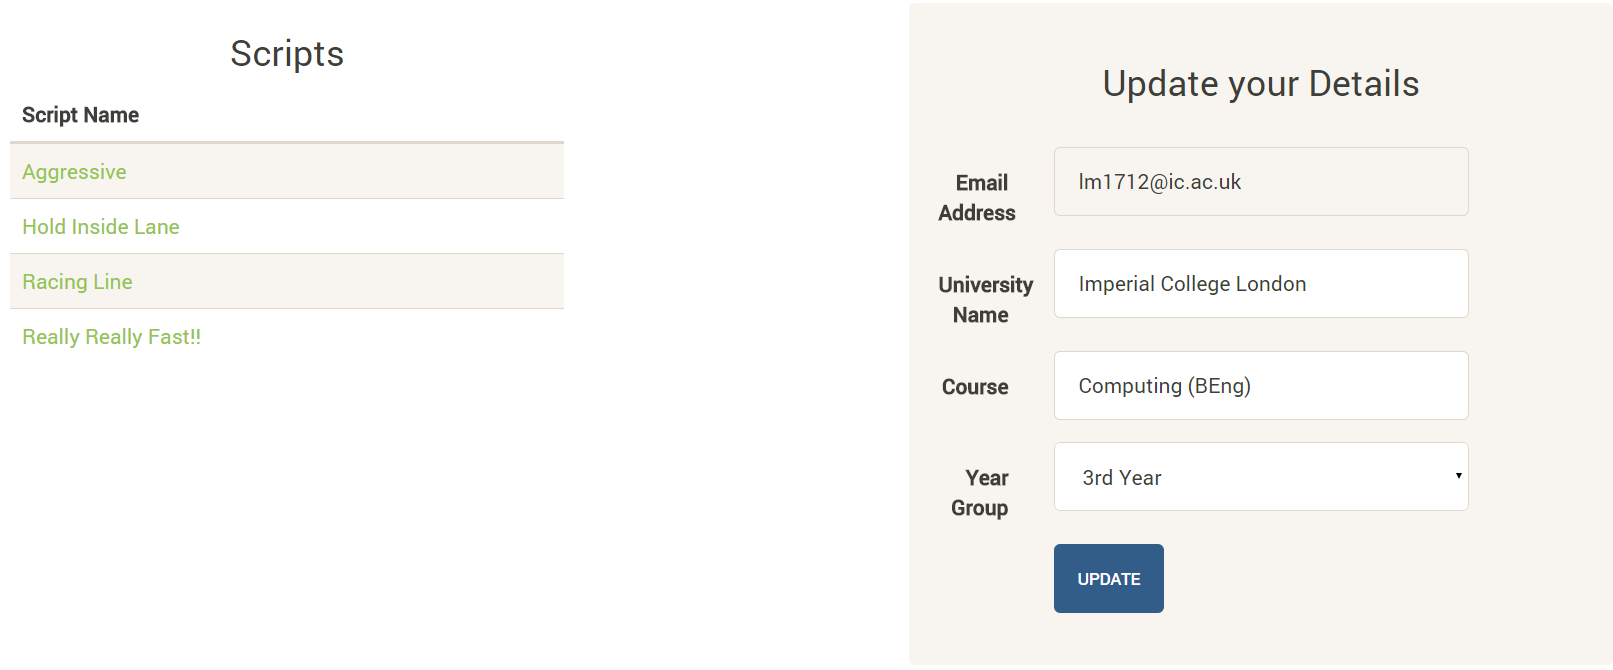
\includegraphics[scale=0.34]{profile}}
User accounts store some optional personal information interested students can fill in. The scripts on the left hand side of the page are owned by the user and can be edited at any time. The admin user can view these details, and see who owns which scripts.

\subsection{Scripts}
\centerline{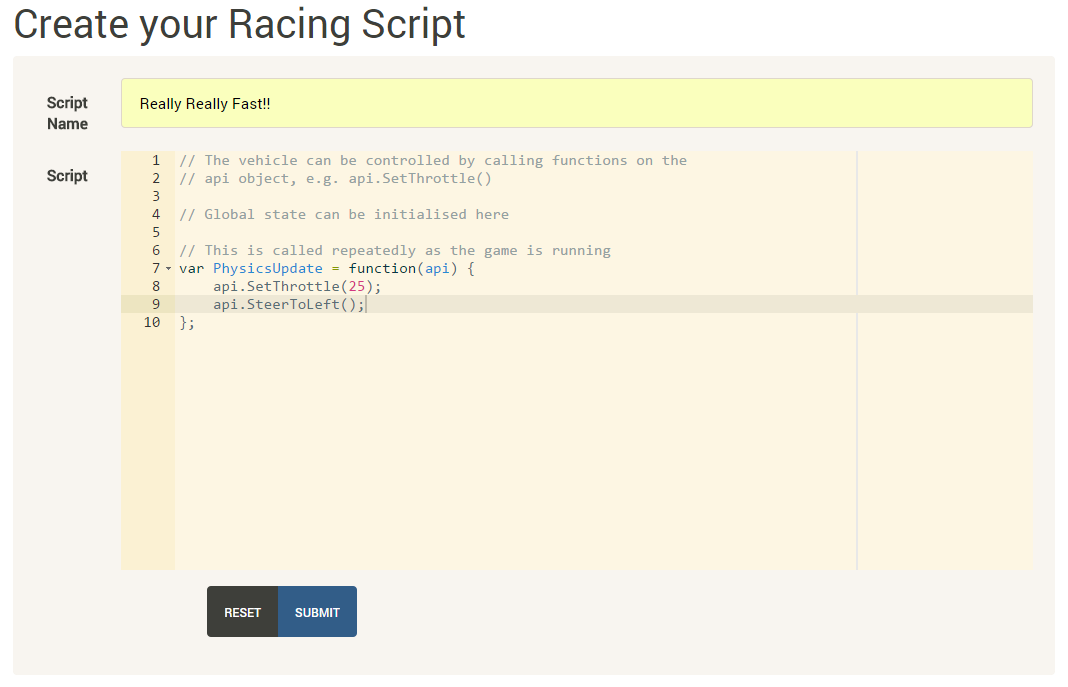
\includegraphics[scale=0.5]{script}}
Scripts can be written in either Coffeescript or Javascript and are very easy to code. Above is a trivial two line script which can be implemented in seconds, and will drive around a track at a constant speed holding the inside lane. There are many more API calls available to design superior scripts with greater complexity, such as using boost, getting proximity of nearby cars, and the determining sharpness of the next corner. Full API documentation is available in appendix A. While editing scripts users can run test races to see how their AI stacks up against others, and to get quick feedback on any changes they make.

\subsection{Races}
\centerline{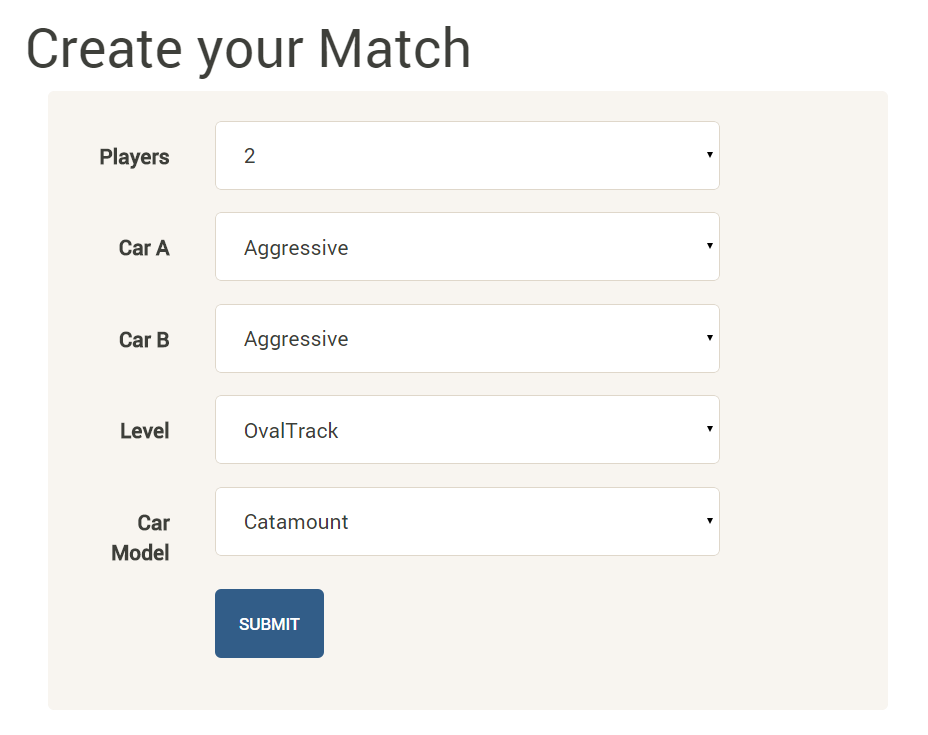
\includegraphics[scale=0.5]{creatematch}}
Creating races allows for a variety of options, including different number of cars and a choice of multiple tracks. Once options have been selected, the race is run in Unity and the users can cheer their scripts on. The camera can move between the different cars and the HUD tracks the lap number and the positions of the cars. At the end of the race the results are sent to the database and the updated leaderboard is shown to the user.

\centerline{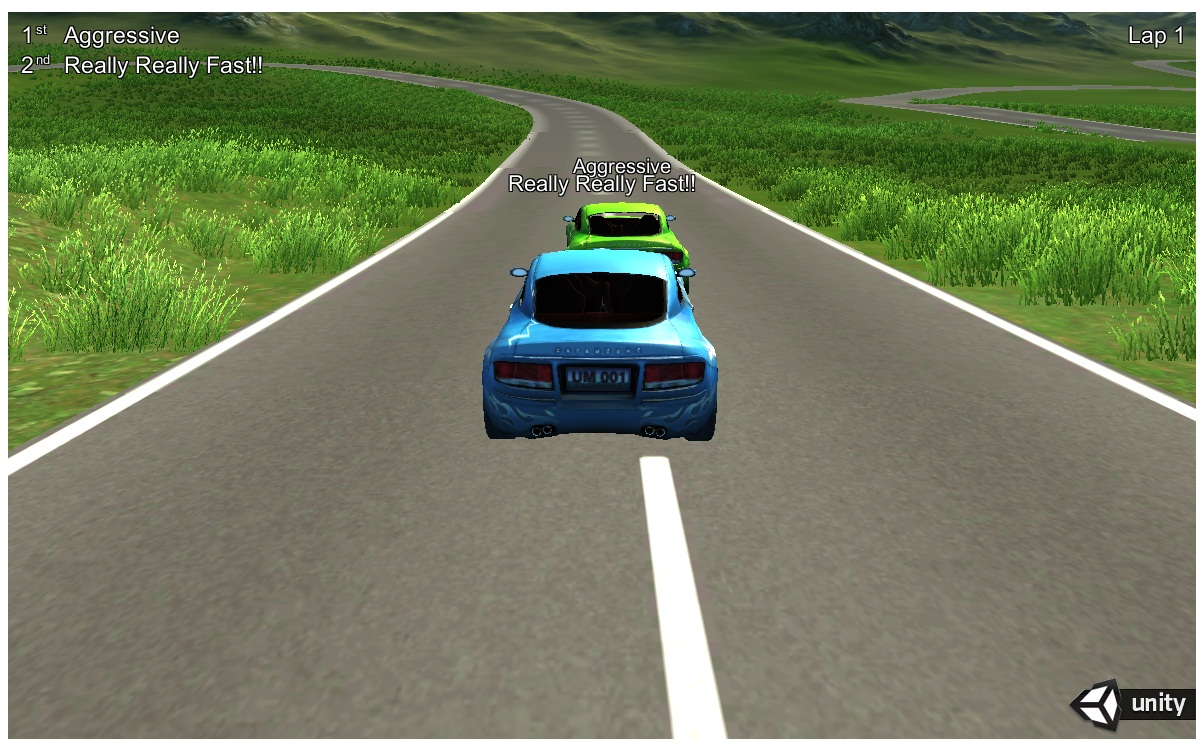
\includegraphics[scale=0.405]{race}}

\subsection{Leaderboard}
\centerline{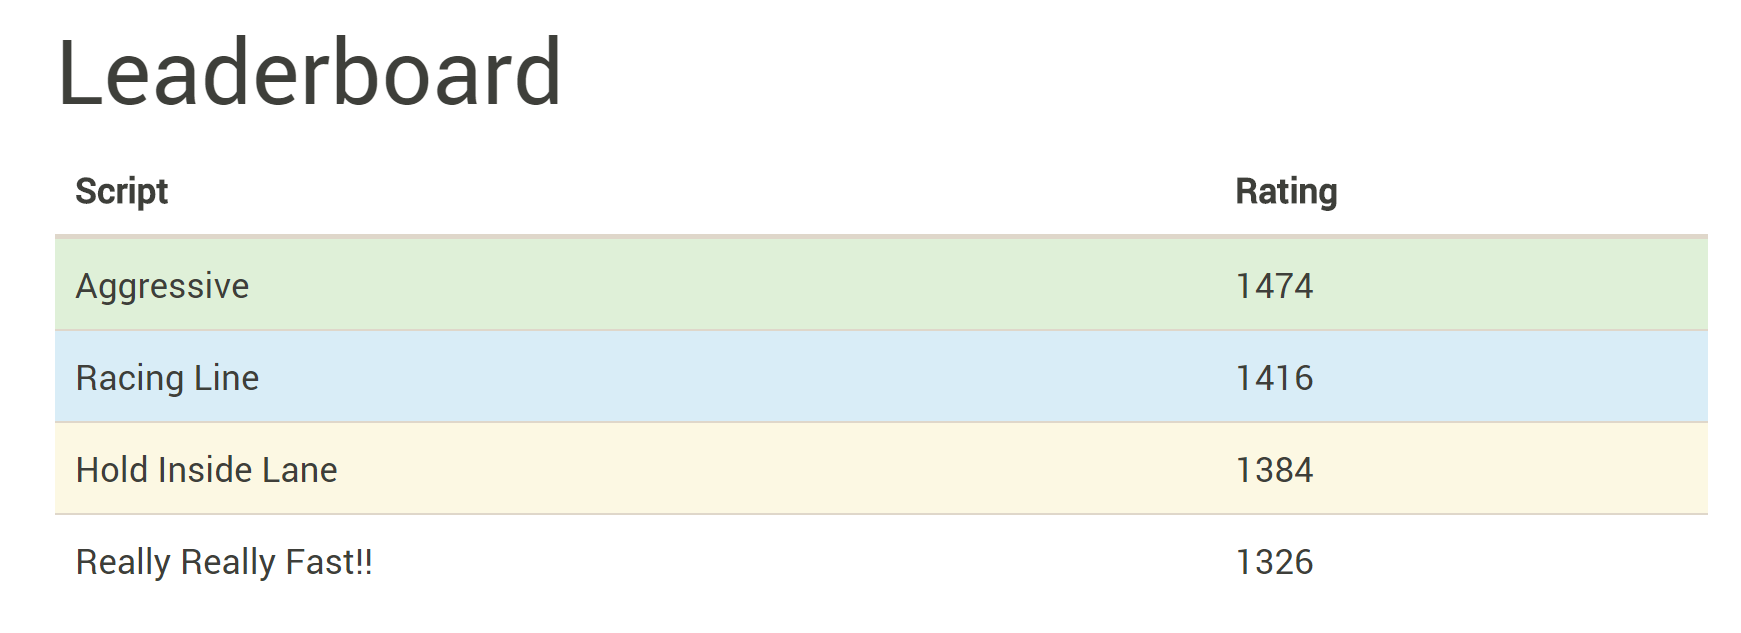
\includegraphics[scale=0.35]{leaderboard}}
A leaderboard displays the Elo ratings of each script, calculated after each race. With enough races the best scripts will rise to the top.
